\chapter{Methods}
\label{c:method}

In the following sections, first a number of typical RNA-Seq and DNA-Seq
pipelines that BioCloud supports are defined and explained. Then the design of
BioCloud is explained by breaking down into two main parts: the website and the
report generator. For the website, the components including account
registration, data sources management, experiment design, and pipeline
execution are described and their roles are illustrated in the website overview
workflow. For the report generator, the workflow is shown to demonstrate how
outputs of each tool is extracted, parsed, and rendered into pre-defined
web-based report templates.



\section{RNA-Seq pipelines}
\label{s:rnaseq-pipeline}

The RNA-Seq analysis pipelines that BioCloud supports are summarized in
Figure~\ref{fig:rnaseq-pipeline}, where some of the tools are shared for
different pipelines. The goal of RNA-Seq analysis is to infer differential
expression of gene or transcripts across different conditions. Based on
different assumptions of the distribution of gene and transcript expression,
three different methods are used: Cufflinks, DESeq2, and kallisto, which yield
FPKM based, count-based, and abundance-based expression value respectively.

\begin{figure}[!htbp]
\centering
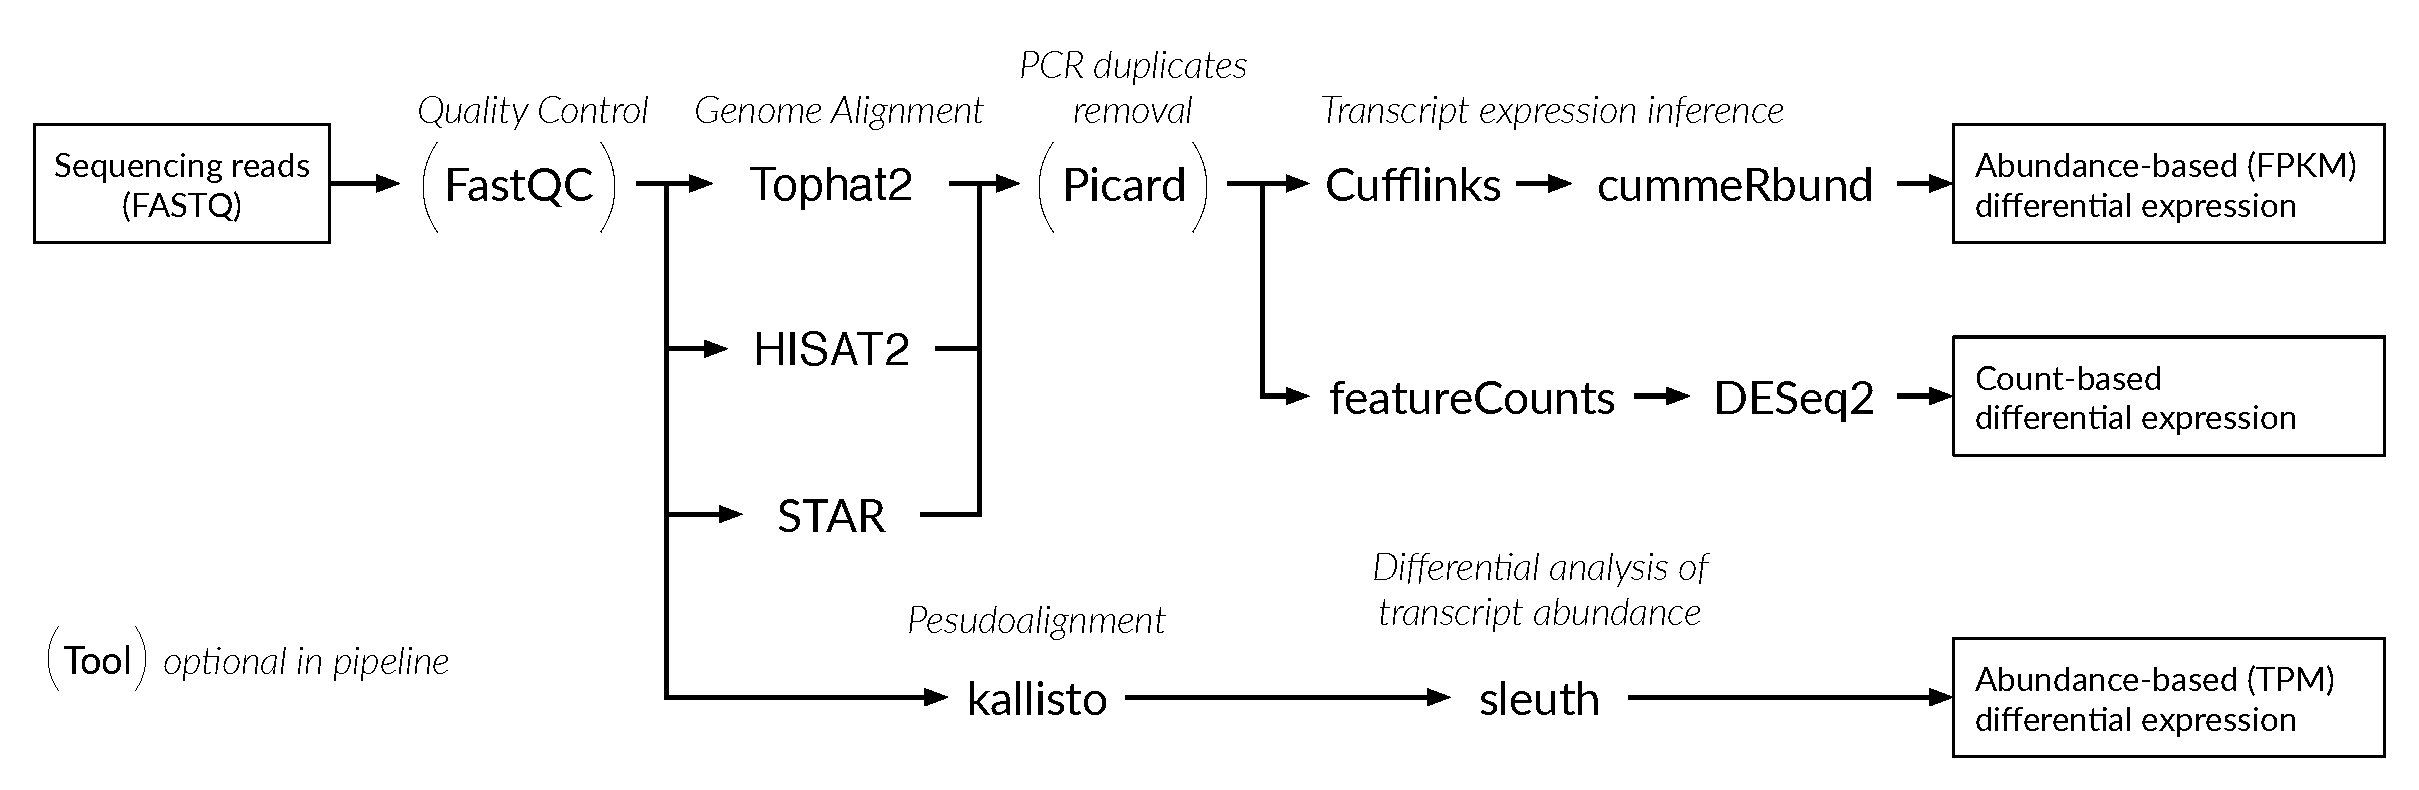
\includegraphics[width=\textwidth]{images/rnaseq_pipelines}
\caption[RNA-Seq analysis pipelines]{RNA-Seq analysis pipelines supported by BioCloud.}
\label{fig:rnaseq-pipeline}
\end{figure}


Cufflinks \cite{trapnell2010:transcript} and its differential analysis method
Cuffdiff \cite{trapnell2013:differential} are best used for gene expression
considering its isoforms, e.g., differential expression on transcript-level.
The output of Cuffdiff can be further visualized using R package cummeRbund
\cite{:cummerbund} from the same development team of Cufflinks. The unit of
expression Cufflinks uses is reads per kilobase of exon per million reads
mapped (FPKM). For DESeq2 \cite{love2014:moderated}, its model analyzes
expression change on gene level using read counts, which cannot be applied to
transcript level analysis. The unit of expression DESeq2 uses is normalized
read counts. The read counts are computed by featureCounts
\cite{liao2014:featurecounts}.  Another popular alternative for computing read
counts is HTSeq \cite{anders2015:htseqa}. HTSeq generally acts the same as
featureCoutns while having slower processing speed so it is not used in
BioCloud.

Both Cufflinks and DESeq2 require genomic location of reads so their analysis
is prepended by the genome alignment step. Three aligners are supported:
Tophat2 \cite{kim2013:tophat2}, HISAT2 \cite{kim2015:hisat}, and STAR
\cite{dobin2013:star}. Though the underlying alignment algorithms of these
tools are different, all of their alignment output in BAM file format can be
used interchangeably by the following expression inference tools. The most
discernible difference is computation time. Given the same execution
environment on a same sequencing sample, Tophat2 takes a hundred times the
computation time of STAR to complete the alignment. HISAT2 uses even slighter
shorter time and significantly less memory than STAR.

Between the genome alignment and expression inference step, an optional step of
removing PCR duplicated reads can be added, which can be done by Picard
\cite{:picard} or Samtools \cite{li2009:sequence}. PCR duplication can occur in
some NGS technology that requires PCR amplification when the given biological
sample has low cDNA template diversity. Filtering out PCR duplication can rule
out the expression bias made by PCR and reduce the computation time due to
fewer reads. However, PCR duplication removal can introduce extra artifact
since no information about PCR duplication can be obtained from the sequencing
data.  That is, the data cannot tell whether a sequence read is PCR duplicated
or not from the sequencing result. Currently the tools label a sequence read as
PCR duplicated if its 5' and 3' genomic position is exactly identical to
another read. Since this empirical rule clamps the dynamic range of gene and
transcript expression, user can choose to skip the step if their NGS technology
does not involve PCR or the PCR duplication effect is negligible.

Contrary to aligning RNA-Seq reads to genome, the concept of pseudoalignment
which does not require actual genome alignment has been brought up in the last
two years. For each sequence read, pseudoalignment finds the most compatible
transcript by sharing the most number of k-mers and use the abundance of k-mers
to infer the estimated the expression of the transcript. By skipping the step
of spliced genome alignment, transcript quantification can be fast and maintain
roughly as accurate as the actual alignment. The idea of pseudoalignment is
first proposed by Salifish \cite{patro2014:sailfish}, formalized and continued
by kallisto \cite{bray2016:nearoptimal} and Salmon \cite{patro2015:accurate}.
Though the differential expression analysis can utilize the existed count-based
analysis tools by rounding the estimated abundance of all transcripts and
summing them to gene level expression, their statistical models on read count
distribution are different. Thus additional tools are developed to provide
better integration with pesudoalignment results, including sleuth
\cite{pimentel2016:differential} and SUPPA \cite{alamancos2015:leveraging}.
Since pseudoalignment is a relatively new concept, only one pipeline is
implemented on BioCloud. User can use kaillisto and sleuth, tools developed by
the same lab, to do pseudoalignment differential expression analysis.

Raw sequence reads are first quality checked using FastQC \cite{:fastqc}.
FastQC provide comprehensive visualization of the quality of sequencing
experiment including per base quality plot, sequencing duplication rate plot,
and adapter sequencing check. FastQC does not affect the content of sequences
thus this step is optional.



\section{DNA-Seq pipelines}

The DNA-Seq analysis pipelines that BioCloud supports are summarized in
Figure~\ref{fig:dnaseq-pipeline}. Some of the tools overlap with RNA-Seq
pipelines which have been already mentioned and described in
Section~\ref{s:rnaseq-pipeline}. To find germline variants, sequence reads are
first aligned to genome by the tool Burrows-Wheeler Alignment (BWA)
\cite{li2009:fast} using its MEM local alignment algorithm.

\begin{figure}[!htbp]
\centering
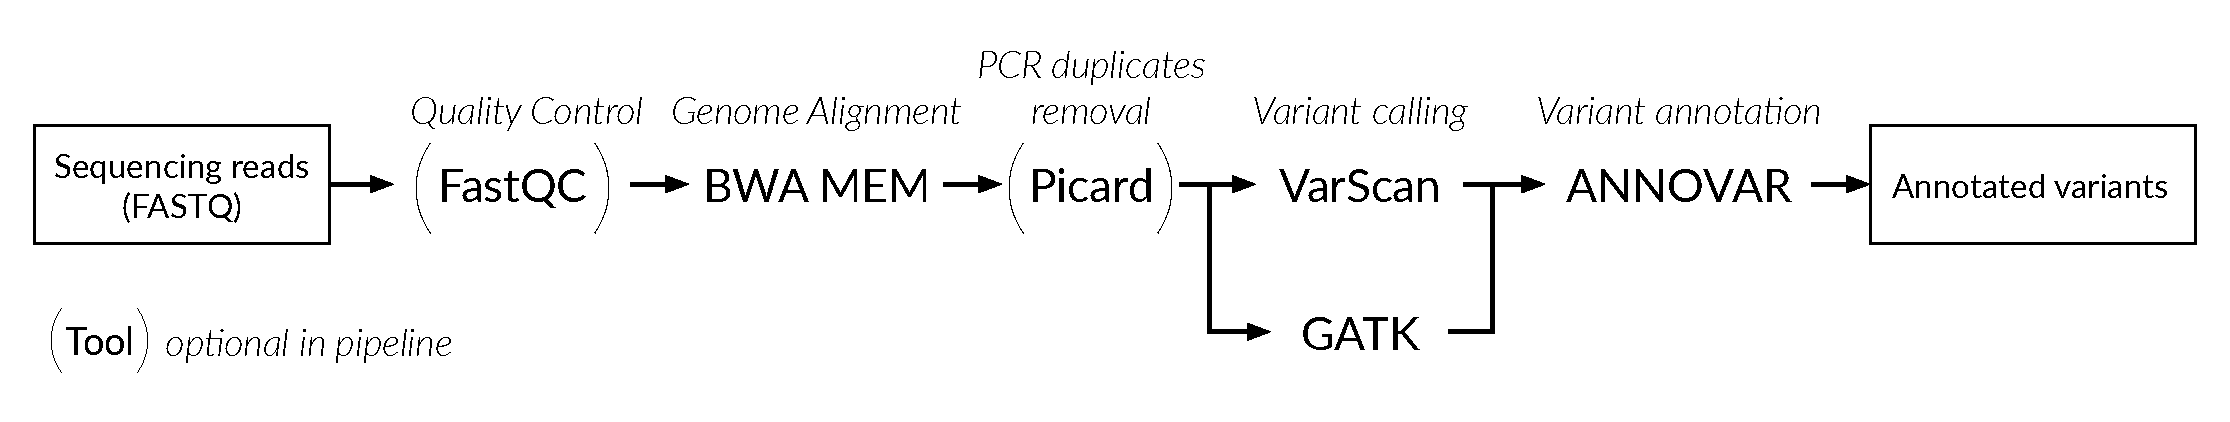
\includegraphics[width=\textwidth]{images/dnaseq_pipelines}
\caption[DNA-Seq analysis pipelines]{DNA-Seq analysis pipelines supported by BioCloud.}
\label{fig:dnaseq-pipeline}
\end{figure}


For variant calling, BioCloud supports two callers: VarScan
\cite{koboldt2012:varscan} and GATK
\cite{vanderauwera2013:fastq,mckenna2010:genome}. To use with VarScan, the
output alignment BAM file is processed by samtools' mpileup subcommand to
compare the aligned reads with genome reference sequence. VarScan take the
mpileup output and determine if it is a significant variant that beyond the
given threshold for each base. To use with GATK, the best practice
\cite{vanderauwera2013:fastq} made by \citeauthor{vanderauwera2013:fastq} is
adopted. However, since our lab does not use GATK for variant calling as
frequently as VarScan, the development to support GATK has been postponed.
Currently existed GATK protocols in our lab are for GATK 1.x, which are
outdated and are not compatible with the newer GATK 2.x.

After variant calling, these variants are further annotated with gene
information, SNP database records, animo acid and protein structure change
predictions by ANNOVAR \cite{wang2010:annovar}. ANNOVAR collects widely used
genome references such as refSeq and Ensembl, annotation databases such as 1000
Genome, dbSNP, ClinVar and COSMIC, and prediction algorithms such as SIFT and
PolyPhen-2. By relying on ANNOVAR, BioCloud don't need to look up each database
and reference on its own, which also reduces the maintaining burden for keeping
all database in use updated.



\section{BioCloud Website}

\subsection{Overview}

\begin{figure}[!htb]
\centering
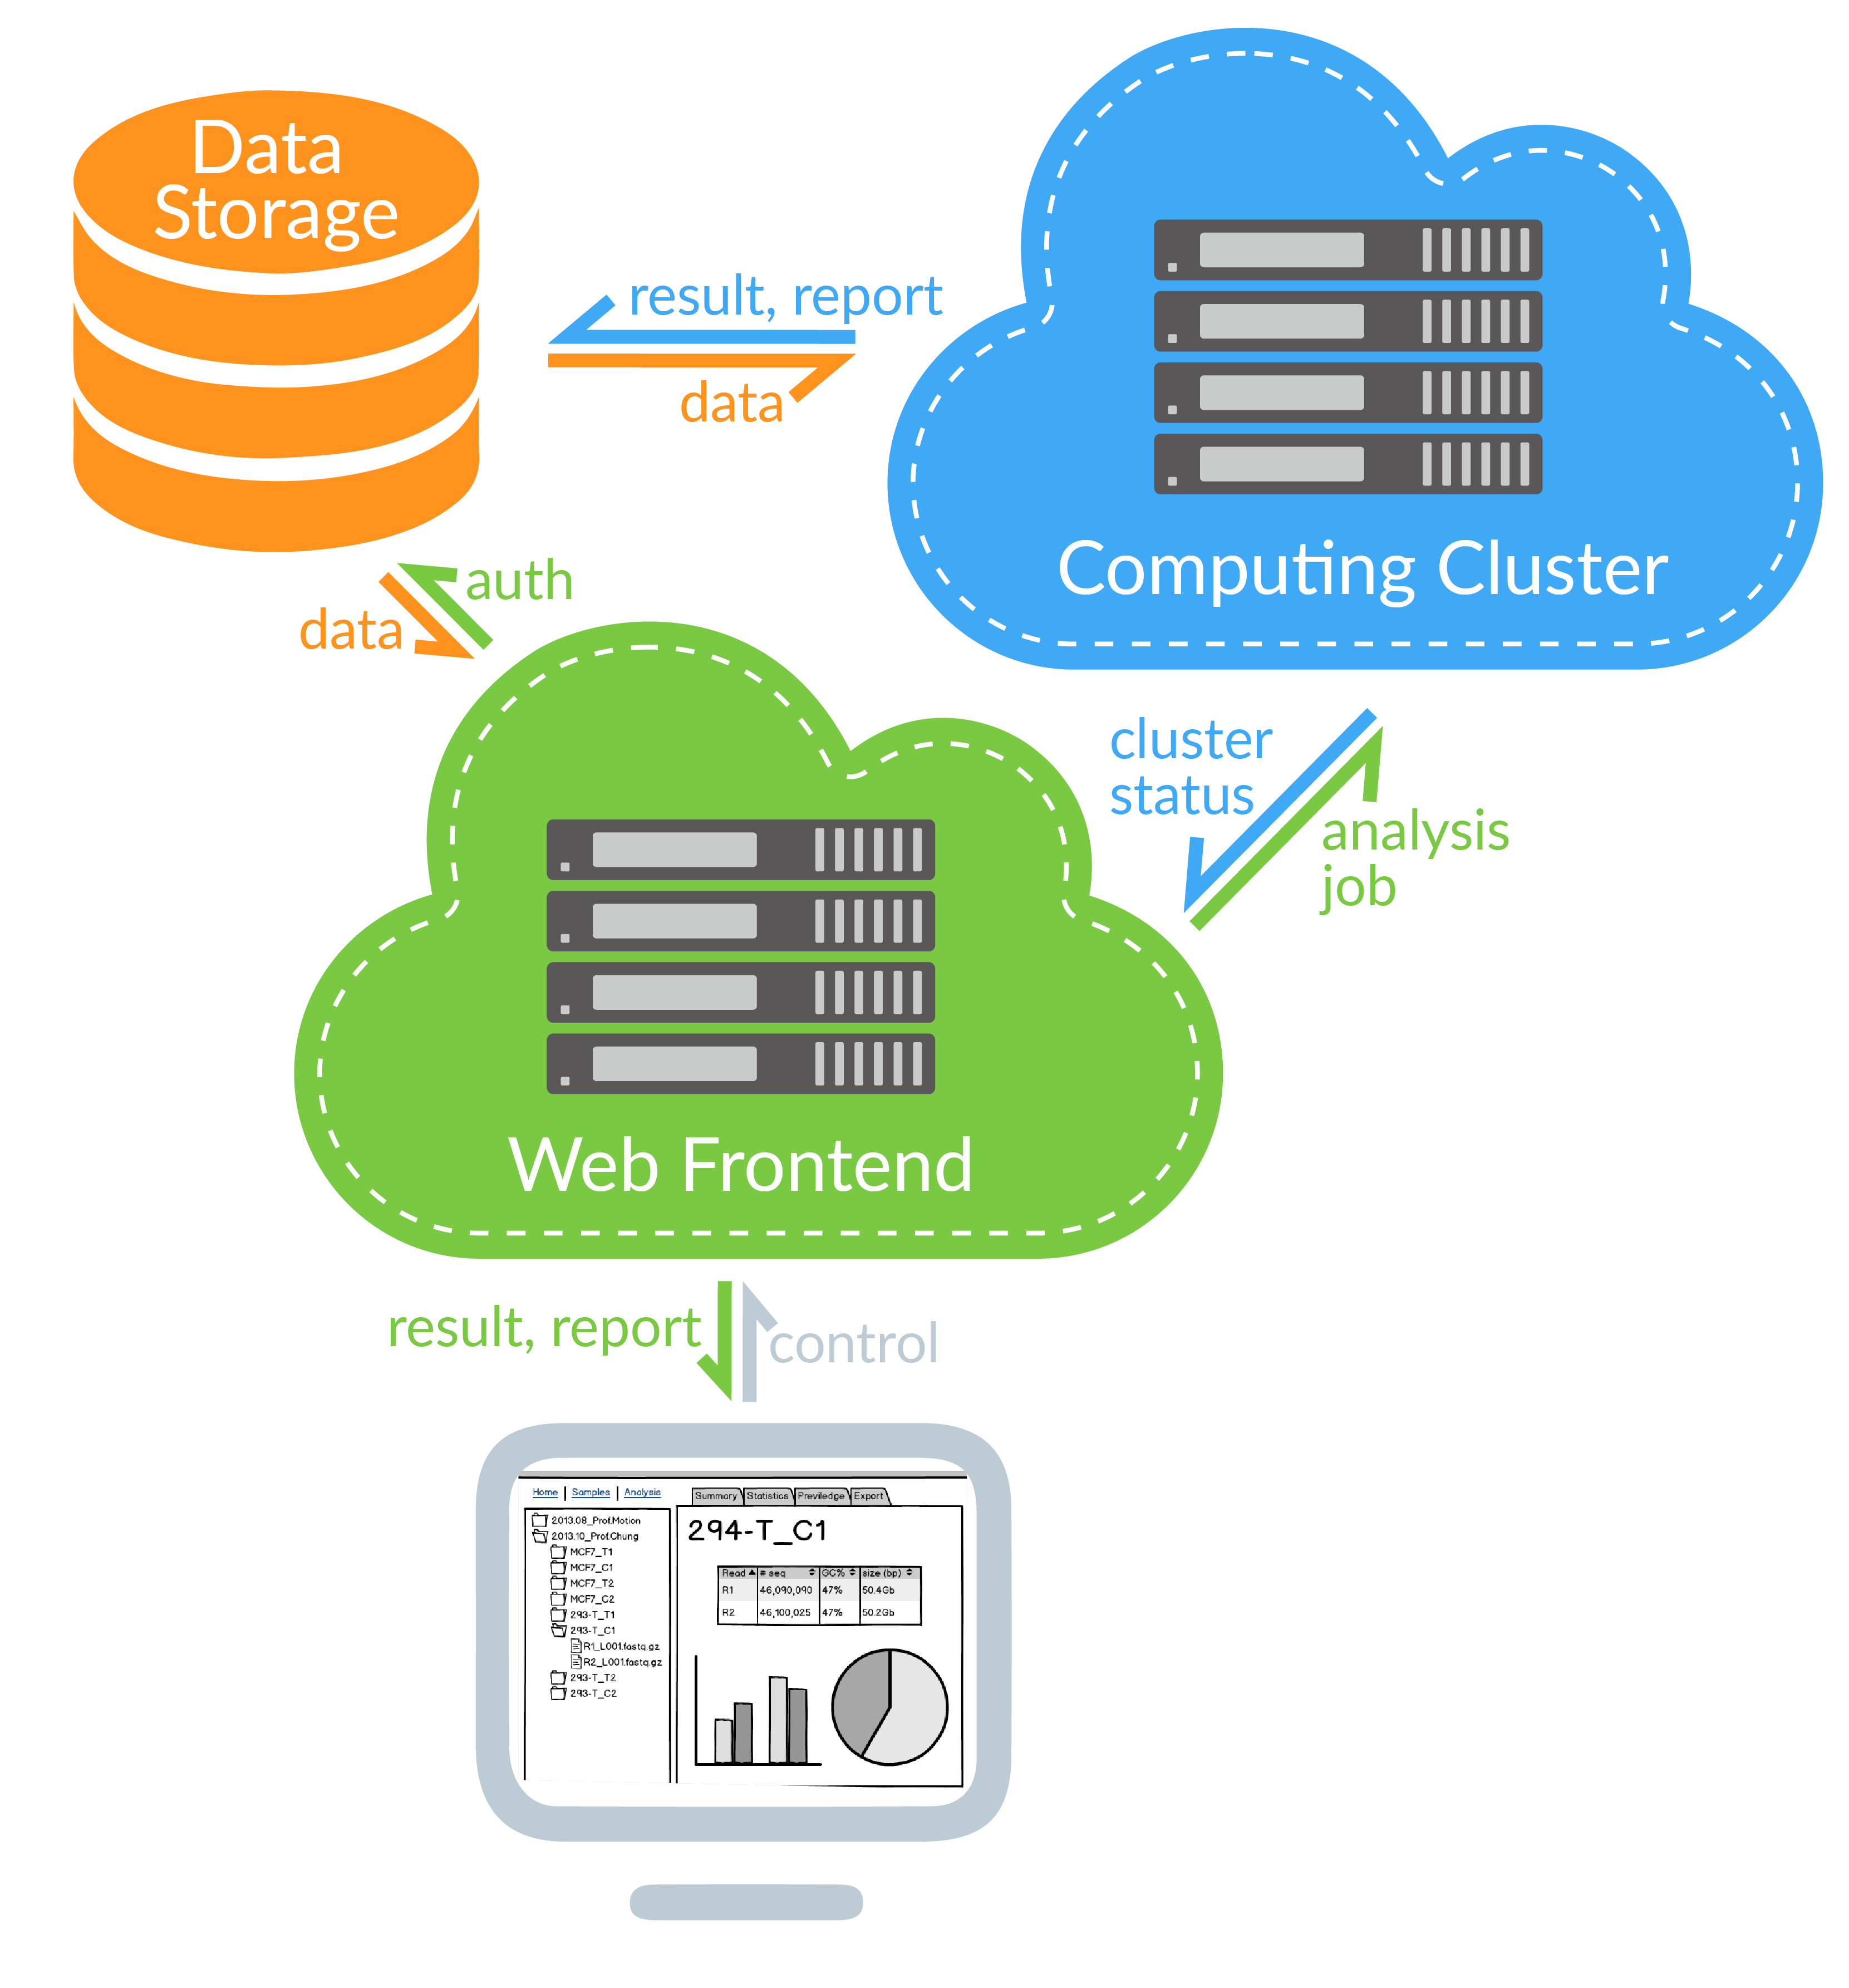
\includegraphics[width=0.75\textwidth]{images/overview_arch}
\caption[BioCloud overview architecture]{Overview of BioCloud architecture.}
\label{fig:overview-arch}
\end{figure}



\begin{figure}[!tb]
\centering
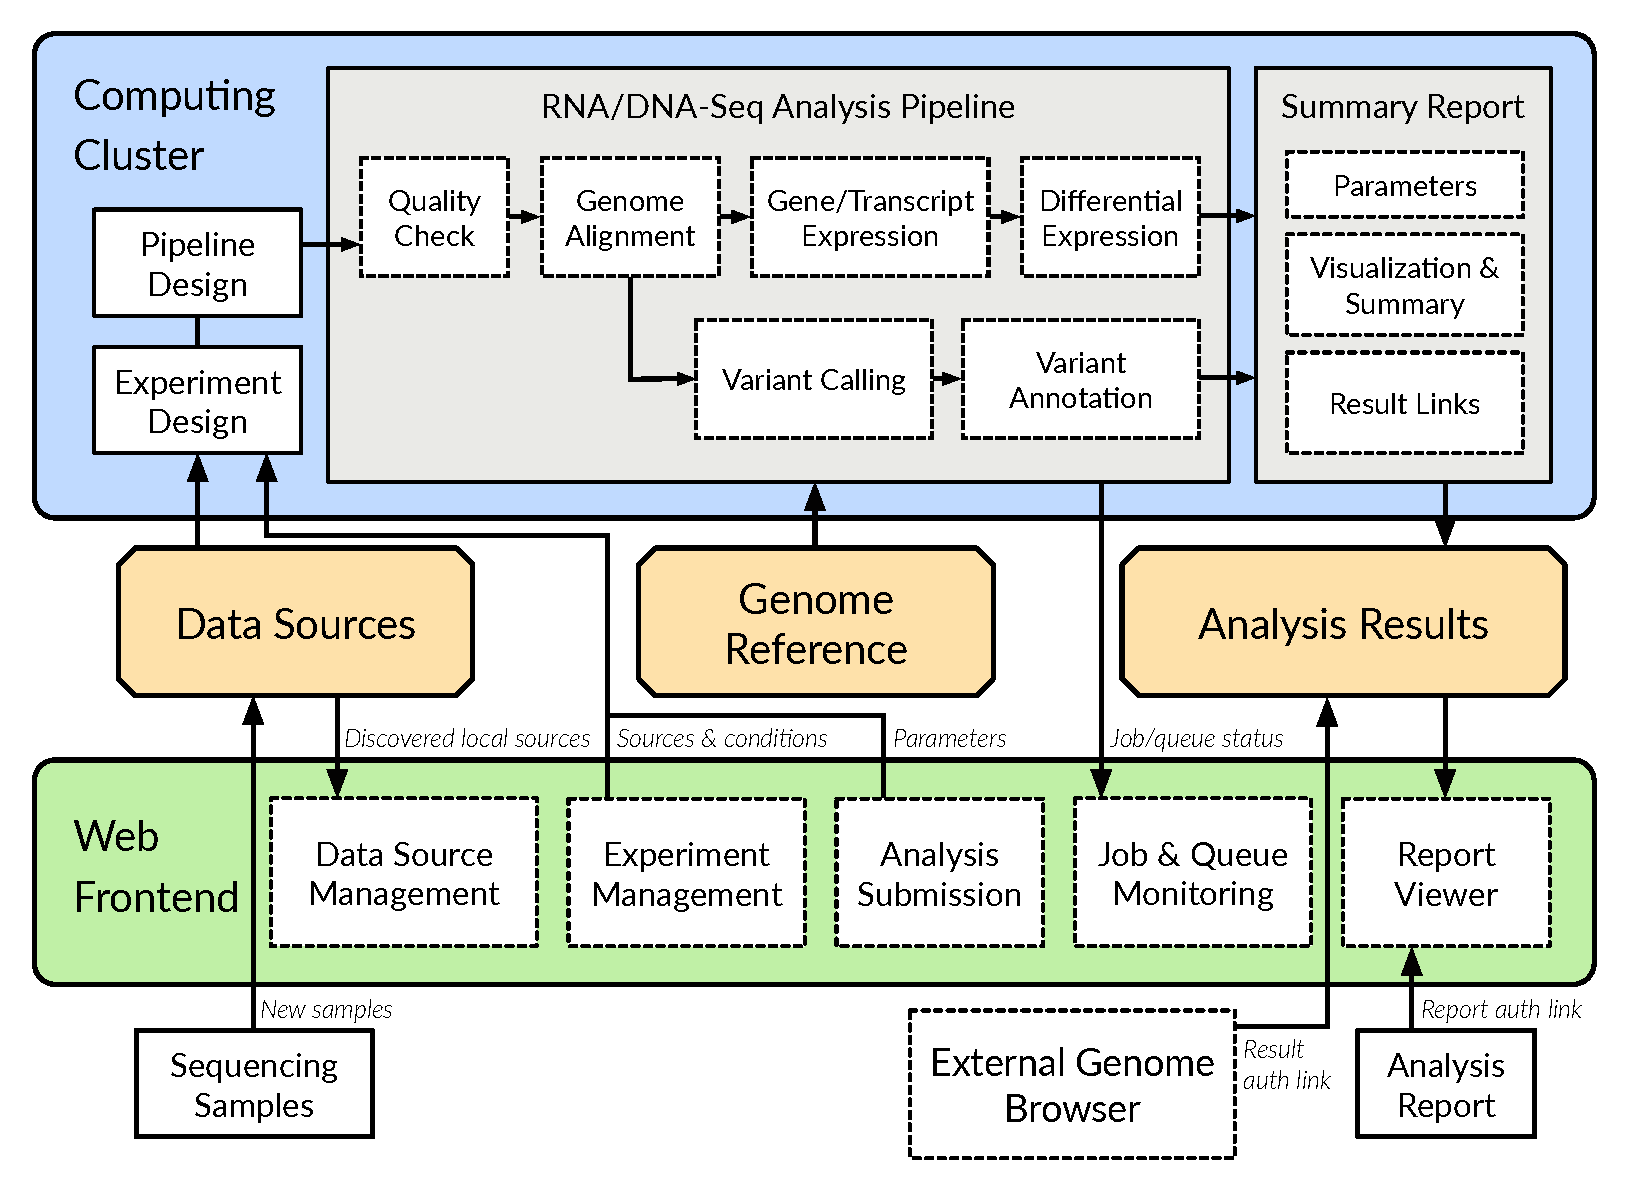
\includegraphics[width=1\textwidth]{images/overview_workflow}
\caption[Overview of BioCloud website workflow]{
    Overview of BioCloud workflow. All operations on data sources, experiments,
    and analysis require user login and thus are isolated by different user
    accounts.
}
\label{fig:overview-workflow}
\end{figure}


\begin{figure}[htbp]
\centering
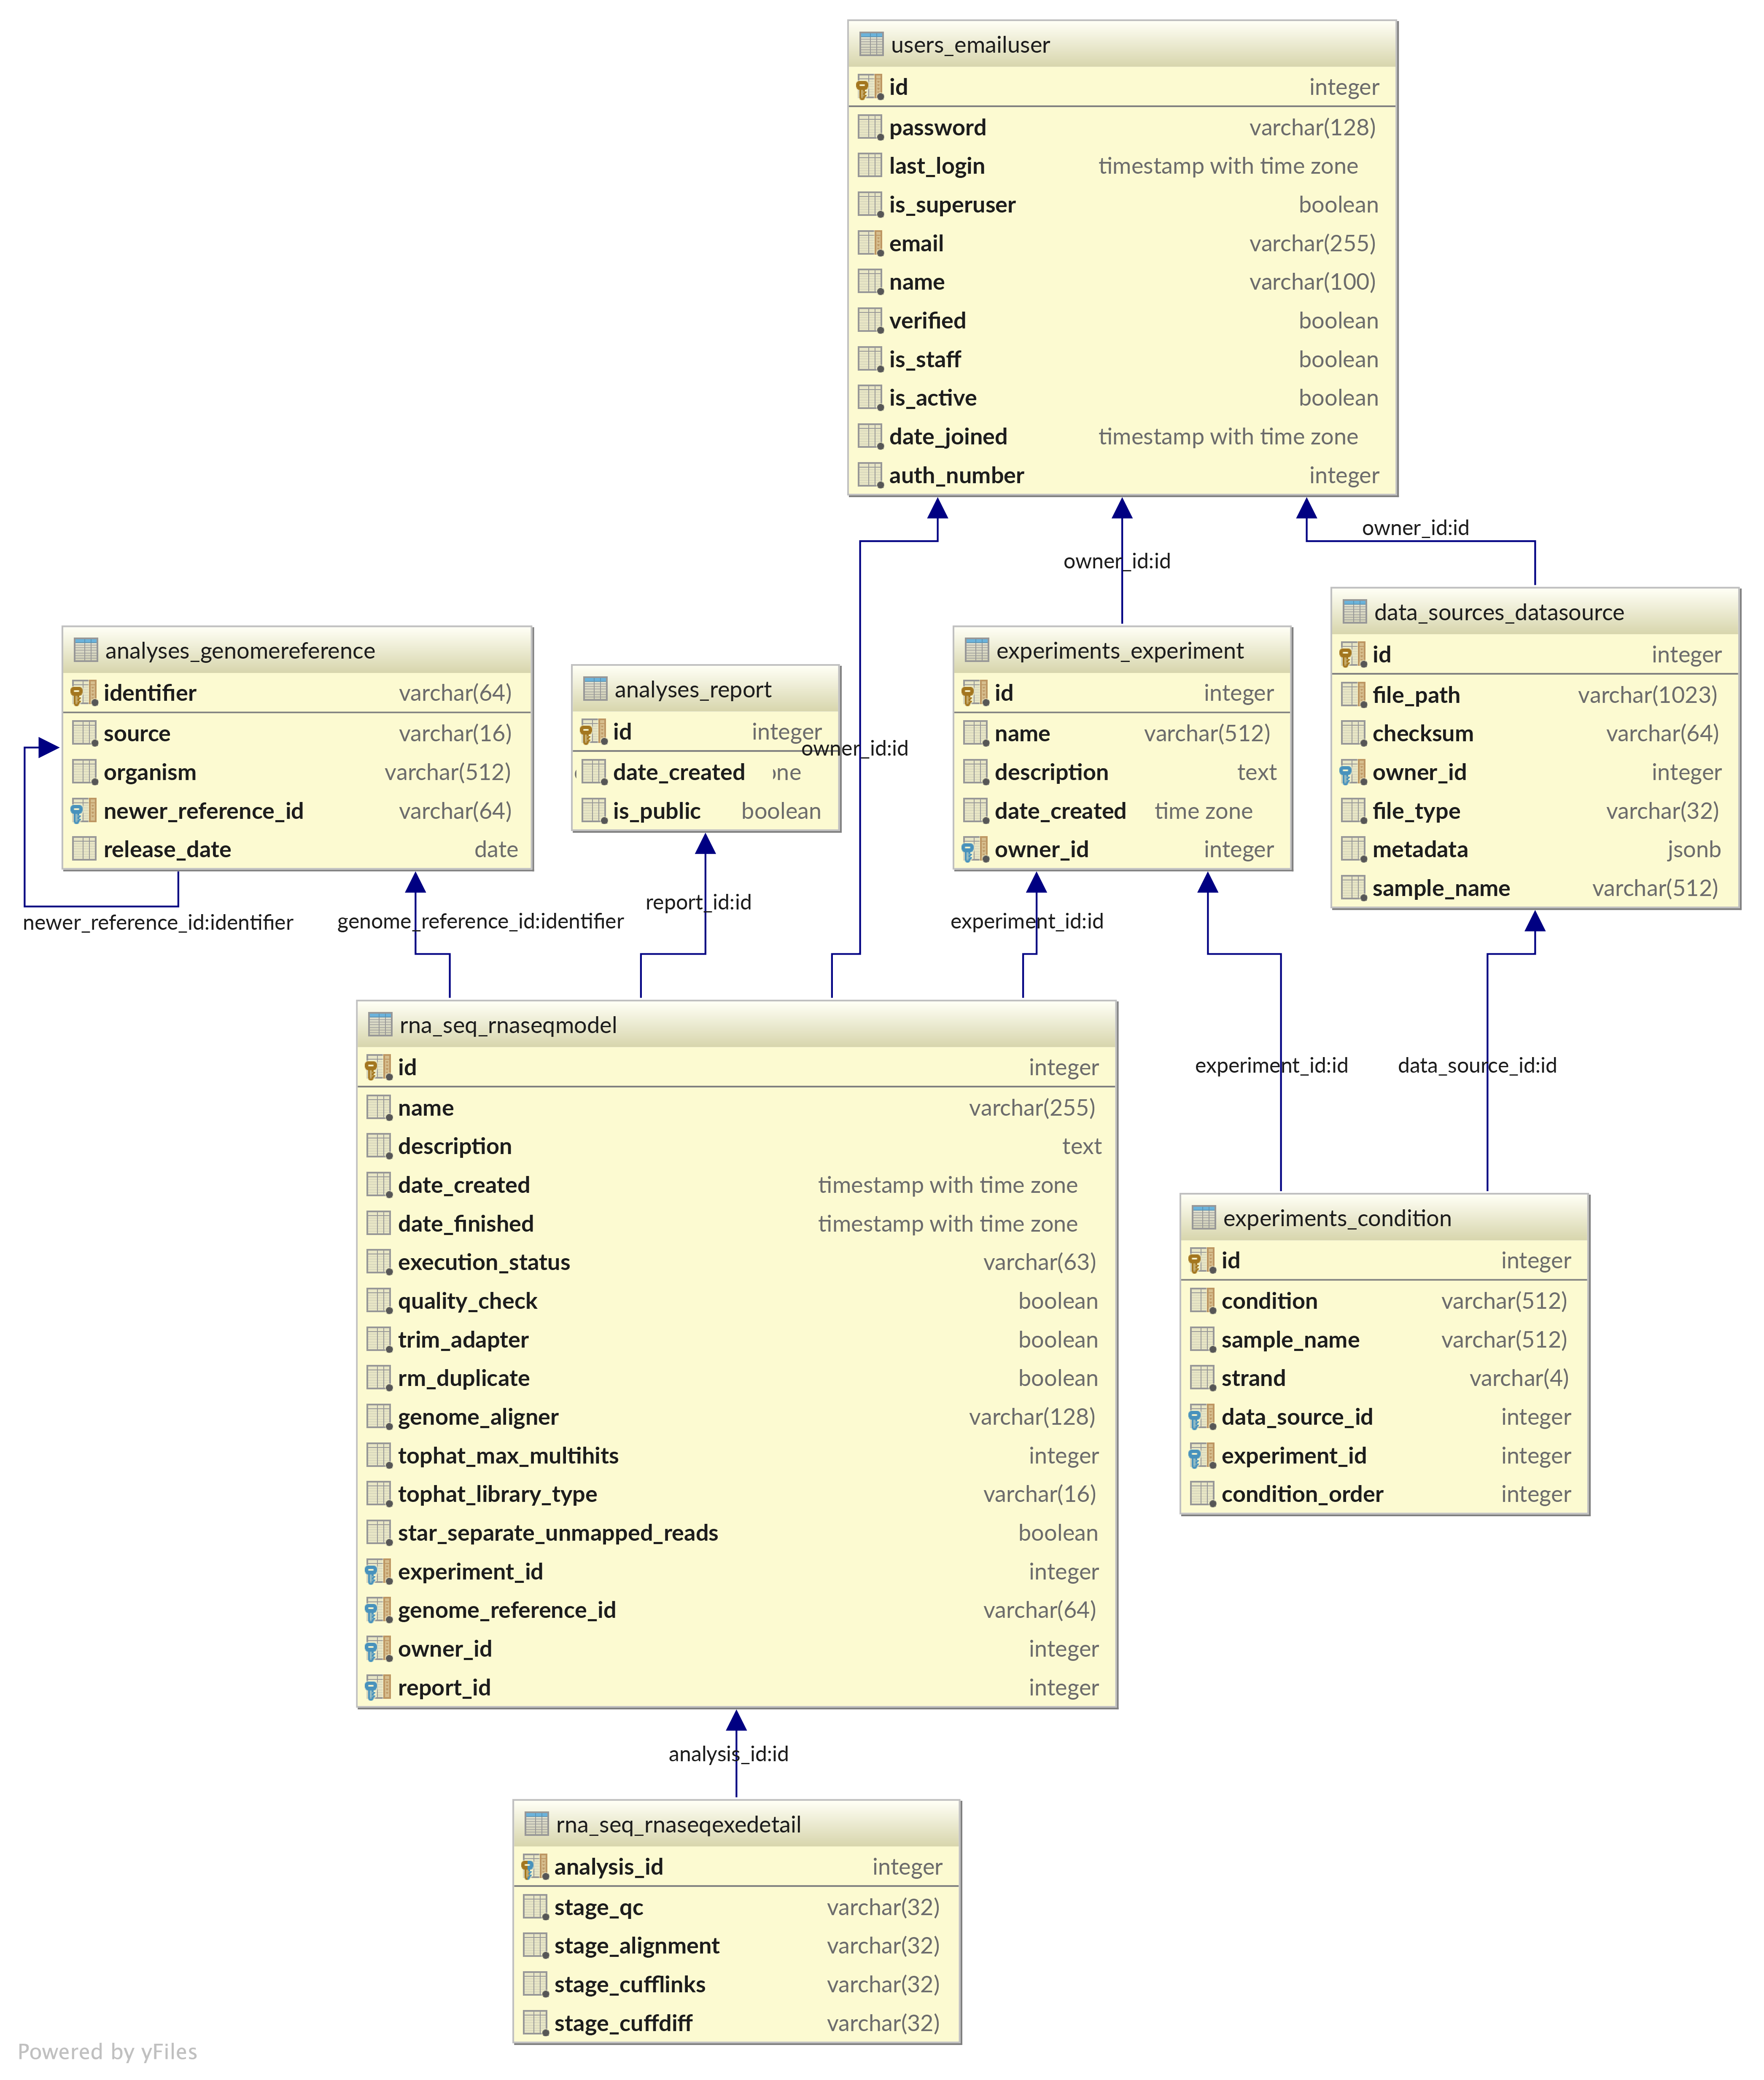
\includegraphics[width=\textwidth]{images/biocloud_erd}
\caption[Entity relation diagram (ERD) of BioCloud database]{
    Entity relation diagram (ERD) of BioCloud database. Here only one analysis
    pipeline of RNA-Seq (table \texttt{rna\_seq\_rnaseqmodel}) is shown for
    simplicity. Tables related with Django web framework internals and job
    queue framework are also omitted.
}
\label{fig:biocloud-erd}
\end{figure}


\subsection{Message authentication and checksum}

Hash-based message authentication code (HMAC)

\subsection{HMAC-based account registration}

\subsection{Experiement design}

\subsection{Genome reference}

\subsection{Analysis submission}

\subsection{Job queue management}

\subsection{Report and result access control}



\section{Report generation}

\subsection{BCReport: result processing framework}



\section{Implementation}

\subsection{Website}

\subsection{Deployment}

\subsection{Report}
% vim: set textwidth=79:
